\chapter{Russian Post Offices in China}  


\subsection{Russian Merchant's Post}

The Russian Merchants' (or Mongolian) Post was a private
enterprise under the protection of the Russian Government initiated
in 1865, about 10 years before the official Russian Post was established
in Mongolia and China. A charge for its service was levied on incoming mail,
payable by the recipient. From January 1872 such mail received the 
standard "Doplatit" (to pay) hs.

\begin{figure}[htbp]
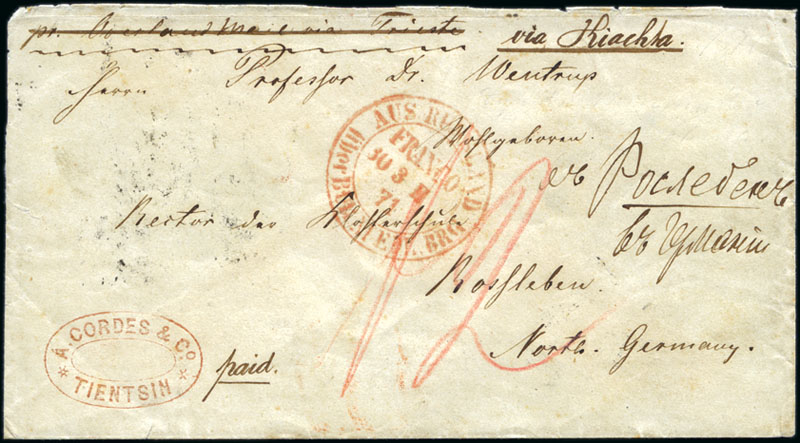
\includegraphics[width=.98\textwidth]{../russian-post-offices-in-china/20000.jpg}
\caption{
Estimate: 15'000 EUR
Price realised: 20'000 EUR 
QUASI OFFICIAL MERCHANTS POST: 1871 Cover from Tientsin to Germany, 
taken to Peking for dispatch by Merchants post as the Russian P.O. 
was not operating from Tienstin at that time, sent via Kyakhta and 
Moscow before arriving in Rossleben, originally franked on the reverse 
with four pen cancelled stamps paying the 30k Merchants rate and 14k 
from Russia to Germany, before the stamps were removed in transit 
between Russia and the German border, noted by German inspector 
who applied "FRANCO" cds with ms "f 2" on front, with ms "China" 
and arrival cds over traces of stamps on reverse, very fine, 
also including 1858 perf. 12 1/2 30k with ms "27 July / 1867 / Pekin" cancel.

The earliest known mail from the Russian Post in China and one 
of the two known cover from the Merchants Post

Note: Described and illustrated in BJRP 94/95 (2006) p.47, Feldman spring 2012
}        
\end{figure}

\subsection{Earliest Known Cover}
The Russian post offices in China were a collection of post offices 
established by Imperial Russia in various cities
of China beginning in 1870.


\begin{figure}[htbp]
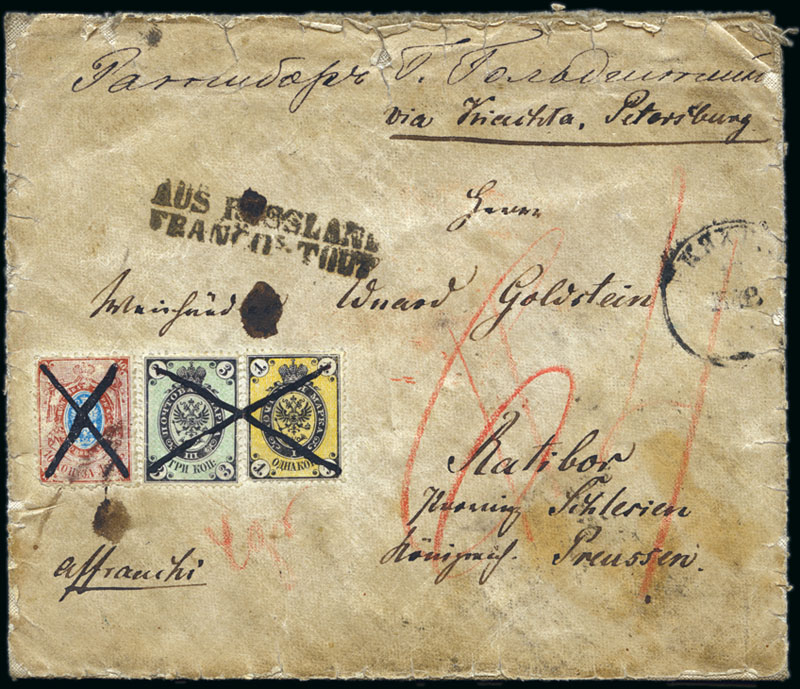
\includegraphics[width=.98\textwidth]{../russian-post-offices-in-china/10000.jpg}
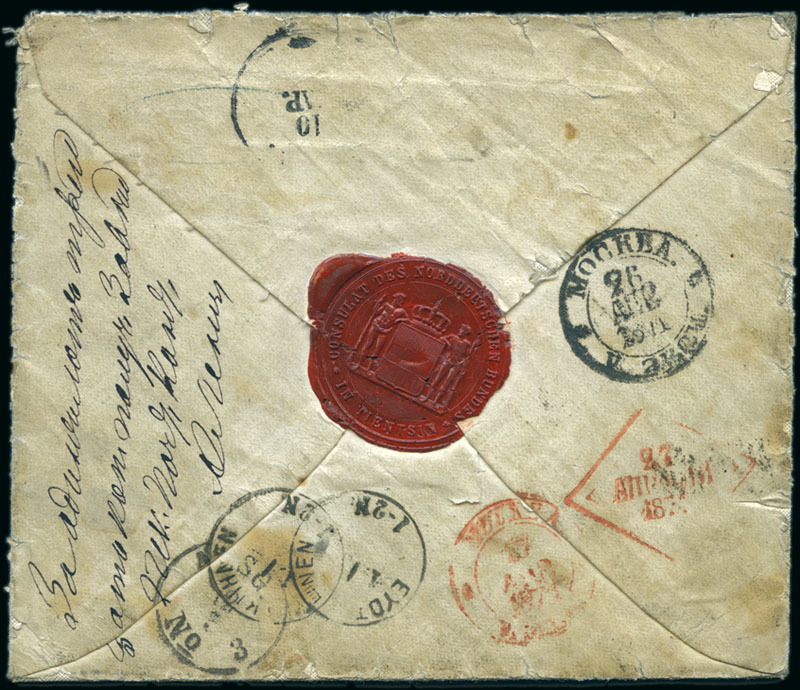
\includegraphics[width=.98\textwidth]{../russian-post-offices-in-china/10000-1.jpg}
\caption{
10000  QUASI OFFICIAL MERCHANTS POST: 1871 Envelope to Ratibor (Prussia)
from the North German Consulate in Tientsin, taken to Peking for conveyance
by Russian Merchants' Post to Russian border at Kyakhta, the fee of 30k paid
in cash with ms note on reverse, Russian 1k, 3k and 10k pen cancelled by
sender for pre-payment of UPU rate from Russia to Prussia, some peripheral
wear, still unique and the earliest known cover bearing Russian stamps in China.
Note: Described and illustrated in BJRP 94/95 (2006) p.45-46
Currently (SAN)...\euro 30,000.00
}  

\end{figure}


\begin{figure}[htbp]
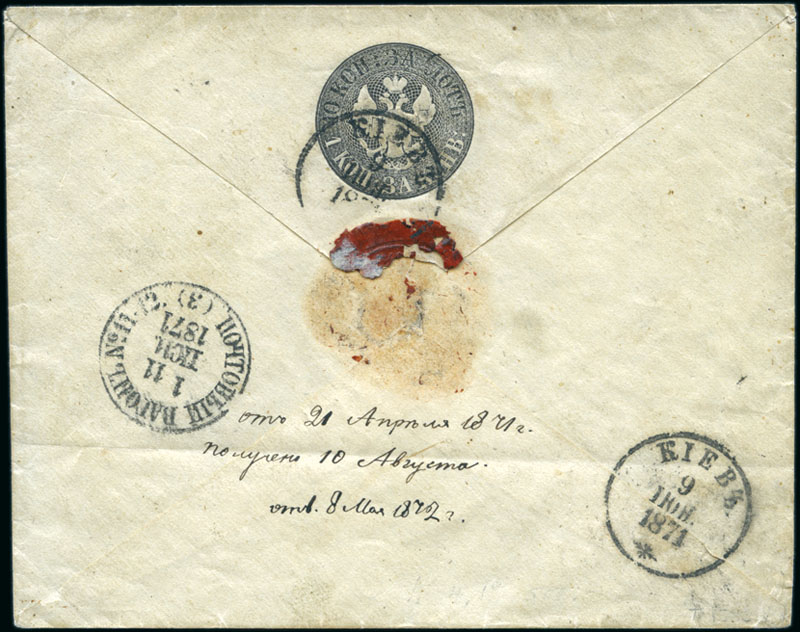
\includegraphics[width=.98\textwidth]{../russian-post-offices-in-china/10001.jpg}
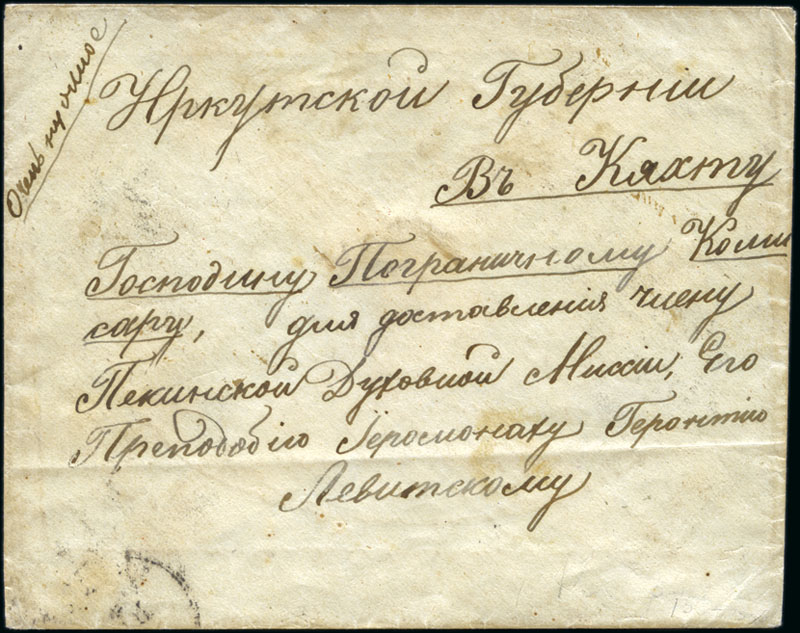
\includegraphics[width=.98\textwidth]{../russian-post-offices-in-china/10001-1.jpg}
\caption{
10001 QUASI OFFICIAL MERCHANTS POST: 1871 Incoming 10k postal 
stationery envelope (1863 issue) sent to the Border Commissar at Kyakhta 
on the Siberia / Mongolia border for transmission to a member of the 
Russian Ecclesiastical Mission at Peking, placed on Postal Wagon No.11-12 
(Kiev-Nizhnii-Novgorod), then taken by Merchants' Post across Mongolia to 
Peking, received 10.8.71 (ms note)
Currently (SAN)...\euro 1,800.00
}        
\end{figure}

\begin{figure}[htbp]
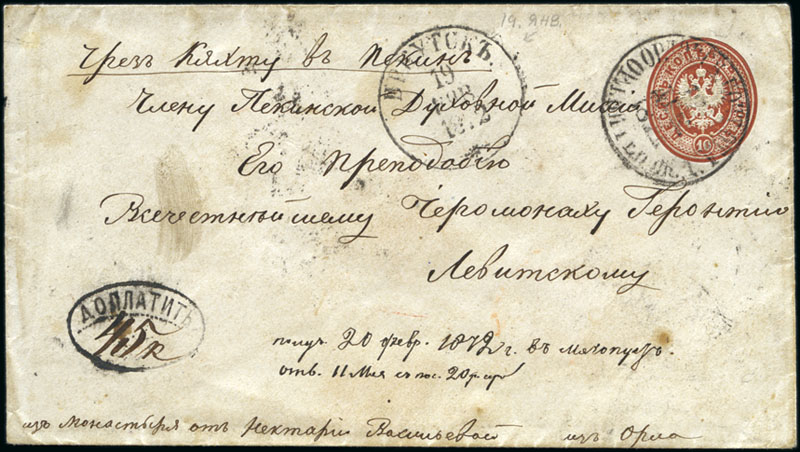
\includegraphics[width=.98\textwidth]{../russian-post-offices-in-china/20001.jpg}
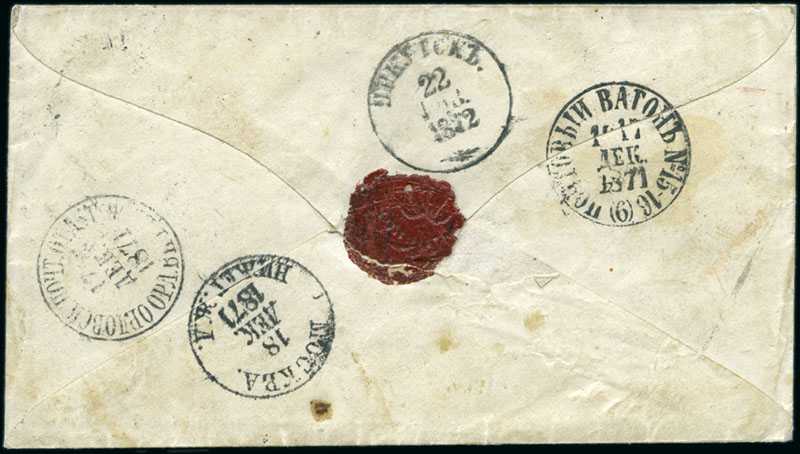
\includegraphics[width=.98\textwidth]{../russian-post-offices-in-china/20001-1.jpg}
\caption{
Estimate: 3'000 EUR
Price realised: 16'000 EUR  April 2012 
QUASI OFFICIAL MERCHANTS' POST: Incoming 1871 Russian 10k postal stationery 
envelope from a convent in Orel to a member of the Ecclestiastical 
Mission at Peking, taken by rail to Nizhnii-Novgrod via Moscow, 
thence by road to the Mongolian border via Irkutsk (Siberia), 
transferred to the Merchants' Post at Kyakhta for conveyance by camel
and donkey to Peking, with several transit bs, oval tax hs from 
Kyakhta for 30k Merchants' Post rate plus 50 percent surcharge for 
underpaid (rated RRR by Hellrigl, possibly unique)
Note: Described and illustrated in BJRP 94/95 (2006) p.45-46
}        
\end{figure}





            